\subsection{Architecture}
\label{sub:sec:solution:arch}

In order to evaluate the proposed backchannel behaviour generation \ac{ML} classifier we require a robotic rapport agent to be tested on human subjects. We propose extending \ac{SERA} framework to manage rapport by providing tools for stimulating positivity, coordination, and mutual attention (similar to Figure~\ref{table:BuildingRapportPlan} on Section~\ref{subsec:Rapport}) enabling flexibility, and reusability in different scenarios. Despite backchannel behaviours being more targeted to enhance mutual attention and coordination, we intend to stimulate positivity as well, by using specific interactional rules.

The architecture that will instantiate the above proposal is depicted in Figure~\ref{fig:rapport:archicture}. The system decision making process is managed by the \textit{Rapport Controller} Module that contains three components: a rule-based and two \ac{ML}-based components.

\begin{figure}
	\centering
	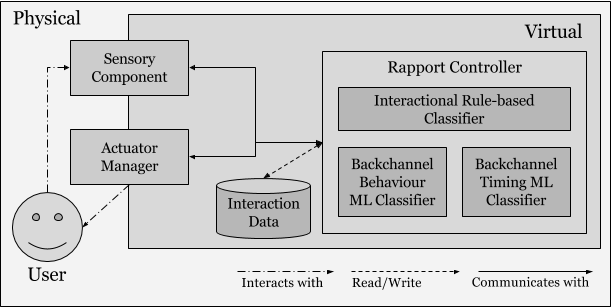
\includegraphics[width=0.75\textwidth]{images/Rapport_archtu.png}
	\caption{Partially decided Rapport Architecture proposal.}
	\label{fig:rapport:archicture}
\end{figure}

The rule-based component is responsible for managing high-level interactional rules that are easier to specify, for example, compliment cooperation actions to stimulate positivity. These rules can be either context specific, or generic enough to be included in other scenarios. The \textit{Interactional Data} data storage depicted in Figure~\ref{fig:rapport:archicture} containts relevant information to manage the interaction.

Two \ac{ML}-based components will handle more complex perceptual states that may arise during the sessions and that would be hard to explicitly define behavioural rules. One module will return correct timings for the generation of backchannels and the other will return the most fitting backchannel behaviour. For example, the first module will suggest that the current instance is appropriate, and the second module will return head nod as the most adequate social behaviour. The retrieved features should be as context independent as possible, including features such as facial expression, head nod frequency, presence of a smile, silence duration, and gaze position. The dominant \ac{ML} classifier is \acf{RL} (Section~\ref{subsec:ReinforcementLearning}) as it was suggested by several authors~\cite{Thomaz2006, Kok2012, Zhao2014, Papangelis2014}.

The \textit{Rapport Controller} will redirect perceptual information collected from the \textit{Sensory Component} and \textit{Actuator Manager} to its component, and will analyse the returned result. From it, the controller will decide which actions should be initiated, maintained or even interrupted. With the bidirectional relationship between the \textit{Rapport Controller}, the \textit{Sensory Component}, and the \textit{Actuator Manager}, we aim to extend \ac{SERA} to support interruptible actions and allow quick adjustments to the agent's behaviour and build better rapport~\cite{Reidsma2011, Visser2014, Kopp2007, Zwiers2011}. For example, similarly to the agent described in Section~\ref{sub:sec:virtualrapport2}, interrupting current speech acts whenever the user starts to speak.

Conflicts may arise between the rule-based component and the \ac{ML}-based components. If the generated behaviours do not conflict with each other, e.g. gaze target and smiling, both actions are executed by the agent. If the generated behaviour conflicts with another, then the \ac{ML}-based components take priority over the rule-based. If there is conflict between two rules, the one with the highest priority takes place (e.g., silence over vocalisation when detecting user's speech).